\chapter{Visual Odometry with RNN}\label{chp:the_model}
% Title ideas: 
% Visual Odometry with Deep Learning
% Visual Odometry
% The Full Visual Odometry Pipeline
	\def\CC{{C\nolinebreak[4]\hspace{-.05em}\raisebox{.4ex}{\tiny\bf ++}}}

	\section{Introduction}
	% Describe the Task
	% Prior Work -> Flownet, DeepVO, VINet
	% 
		The bulk of this chapter and the experiments that follow in chapter~\ref{chp:experiments-and-results} are based on the work of \cite{wang2017deepvo}.
		At the time of writing this thesis, they have not released the source code of their implementation.
		Therefore, the aim of this chapter is to study and re-implement the ideas presented in their paper and to further expand on it.
		To reiterate, the task we try to solve in this thesis is Visual Odometry (VO).
		Given a video, the output of the system should be a sequence of poses describing the camera motion in the video.
		\citeauthor{wang2017deepvo} propose a Deep Learning approach that makes use of an RNN to handle a video of arbitrary length and learn dependencies over time.
		What follows is a detailed description of the proposed Deep Learning pipeline for VO.
		
	\section{Datasets}
		Every machine learning project starts with the collection and assessment of data.
		Data is what drives machine learning, and often it is also a limiting factor.
		Generally, the more data, the better the learning process.
		However, it is not always easy to get the desired amount and quality.
		For VO, the videos need to be recorded manually, which is very time consuming.
		Not only that, but in our supervised setting, accurate per-frame pose annotations are required.
		Therefore we have two main quality requirements for the data in VO: Accurate ground truth pose and realistic image quality.
		The following subsections describe the different datasets that are used in this thesis.
		
		\subsection{KITTI}
			KITTI from the Karlsruhe Institute of Technology (\cite{geiger2013vision}) is a dataset that contains many videos captured from the roof of a driving car.
			Some example images are shown in figure~\ref{fig:example-images-from-KITTI}.
			Each video frame is labeled with ground truth data such as camera pose and 3D points from a velodyne laser scanner.
			The camera pose was obtained by combining the data from GPS and an IMU (inertial measurement unit) that was mounted to the car.
			The dataset has around 43k stereo pairs of images with size $1226 \times 370$ pixels captured at a frame rate of about 10 fps.
			For the experiments in this thesis, only the images from the left camera are used.
			The dataset is divided into 22 sequences, each captured at a different location in the metropolitan area of Karlsruhe, Germany.
			For the public, the ground truth is only available for the first 11 sequences.
			The rest of the data is intended to be used for submissions to the KITTI Vision Benchmark Suite\footnote{\url{http://www.cvlibs.net/datasets/kitti/eval_odometry.php}} 
			online.
			In the experiments here, only the sequences 0 to 10 are used and divided into training- and test sets, which amounts to around 23k images.
			\begin{figure}
				\def\imwidth{5.9cm}
				\centering
				\begin{subfigure}[b]{0.5\linewidth}
					\centering
					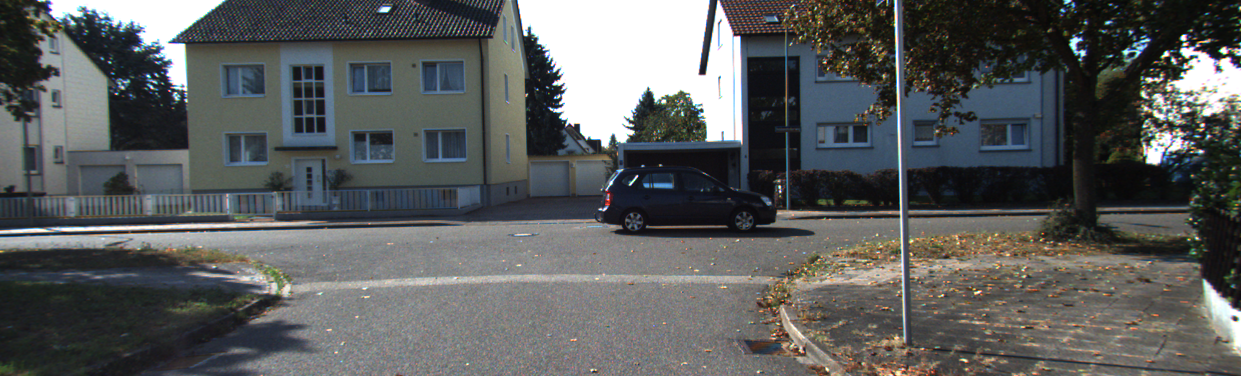
\includegraphics[width=\imwidth]{Data/KITTI/intersection}
				\end{subfigure}\hfill%
				\begin{subfigure}[b]{0.5\linewidth}
					\centering
					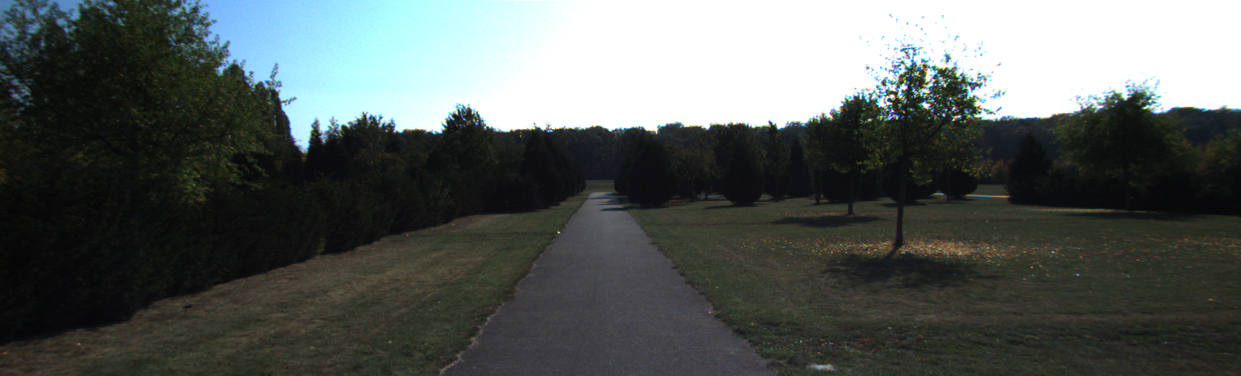
\includegraphics[width=\imwidth]{Data/KITTI/open-field}
				\end{subfigure}\hfill%
				\\
				\vspace{0.1cm}
				\begin{subfigure}[b]{0.5\linewidth}
					\centering
					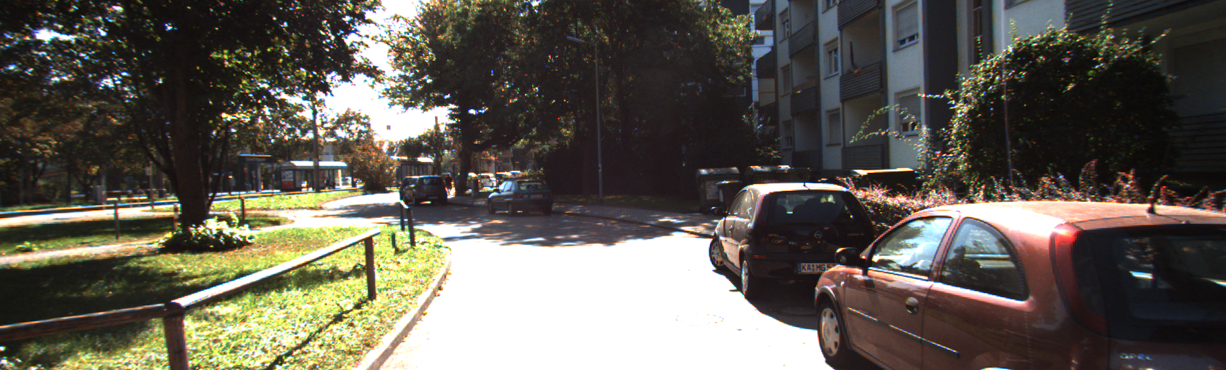
\includegraphics[width=\imwidth]{Data/KITTI/reflections-on-cars}
				\end{subfigure}\hfill%
				\begin{subfigure}[b]{0.5\linewidth}
					\centering
					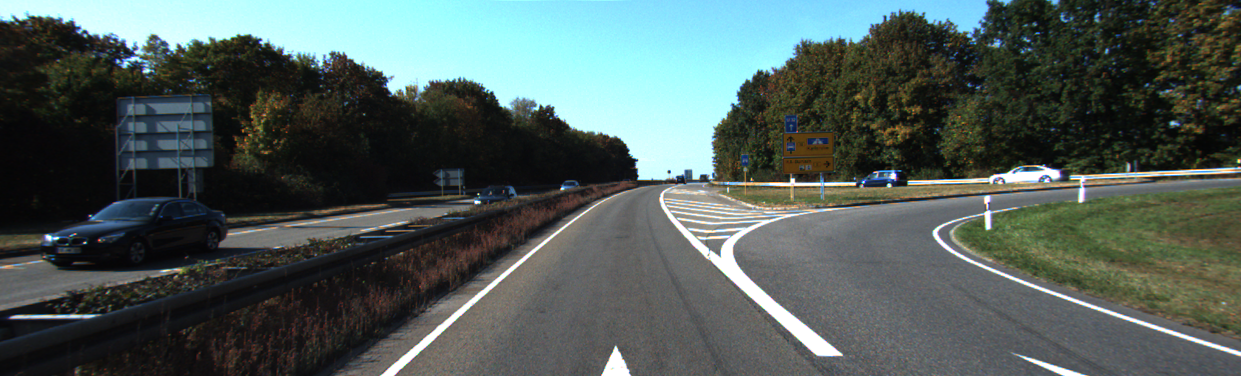
\includegraphics[width=\imwidth]{Data/KITTI/highway}
				\end{subfigure}\hfill%
				\caption[Example images from the KITTI dataset]
						{Example images from the KITTI dataset.
						 The pictures show wide open areas, narrow streets, reflections and moving cars.
						 The videos were captured with a camera mounted on top of a car.
						 \label{fig:example-images-from-KITTI}}
			\end{figure}
		
		\subsection{VIPER}
			The VIPER dataset from \cite{richter2017playing} contains a mix of car driving and walking sequences, but all data was generated synthetically from the video game Grand Theft Auto 5 (GTA V) for PC released in April 2015.
			With around 254k frames it is significantly larger that the KITTI dataset.
			There is a variety of ground truth data available, including camera pose, semantic class labels and 3D object bounding boxes.
			The camera poses have been directly extracted from the game engine and are therefore fully accurate, while other data such as the semantic labels were generated in a post-processing step.
			VIPER is subdivided into training, test, and validation sets with 134k, 70k, and 50k frames respectively.
			The splits contain diverse scenes at day and night across different scene types such as urban, suburban under various weather conditions.
			The videos were captured at a frame rate of 15 fps.
			
		\subsection{GTA V}
			The GTA V dataset, as presented in figure~\ref{fig:example-images-GTAV}, was created specifically for this thesis shortly before the VIPER dataset by \citeauthor{richter2017playing} was made public.
			Third party ``modding" tools%
			\footnote{\url{http://www.dev-c.com/gtav/}}
			had to be used to extract the camera pose information because the game developers do not intend users to modify the game files and only provide binaries for executing the software.
			The tool allows one to inject a user defined \CC\@ function to run code in a separate thread next to the game engine with access to variables such as the camera matrix, player- and world properties and more.
			The tool%
			\footnote{\url{https://github.com/awaelchli/GTA-V-Camera-Tracker}} 
			developed for this thesis streams the camera orientation and location to an output file with timestamps for each recorded pose.
			The video is recorded parallel to the pose with an external program called \emph{NVIDIA ShadowPlay}.
			Although both the recording of pose and video start synchronously, the rate at which the pose is queried is higher than the frame rate of the recorded video.
			Hence, the poses written to the output file were interpolated using the timestamps to match the 30 fps video recording.
			
			The dataset has a total of 470k frames of walking in first-person perspective.
			The sequences contain many factors of variation in form of weather changes (cloudy, sunny, night), dynamic motion of cars on the street or people on the sidewalk, different environments (urban, suburban, rural) and changes in speed (standing, walking, running).
			Although this dataset contains more video data compared to VIPER, it has only pose annotations.
			\begin{figure}
				\def\imheightv{2.2}
				\def\imheight{\imheightv cm}
				\def\imwidth{\fpeval{16/9*\imheightv}cm}
				\centering
				\begin{subfigure}[b]{0.33\linewidth}
					\centering
					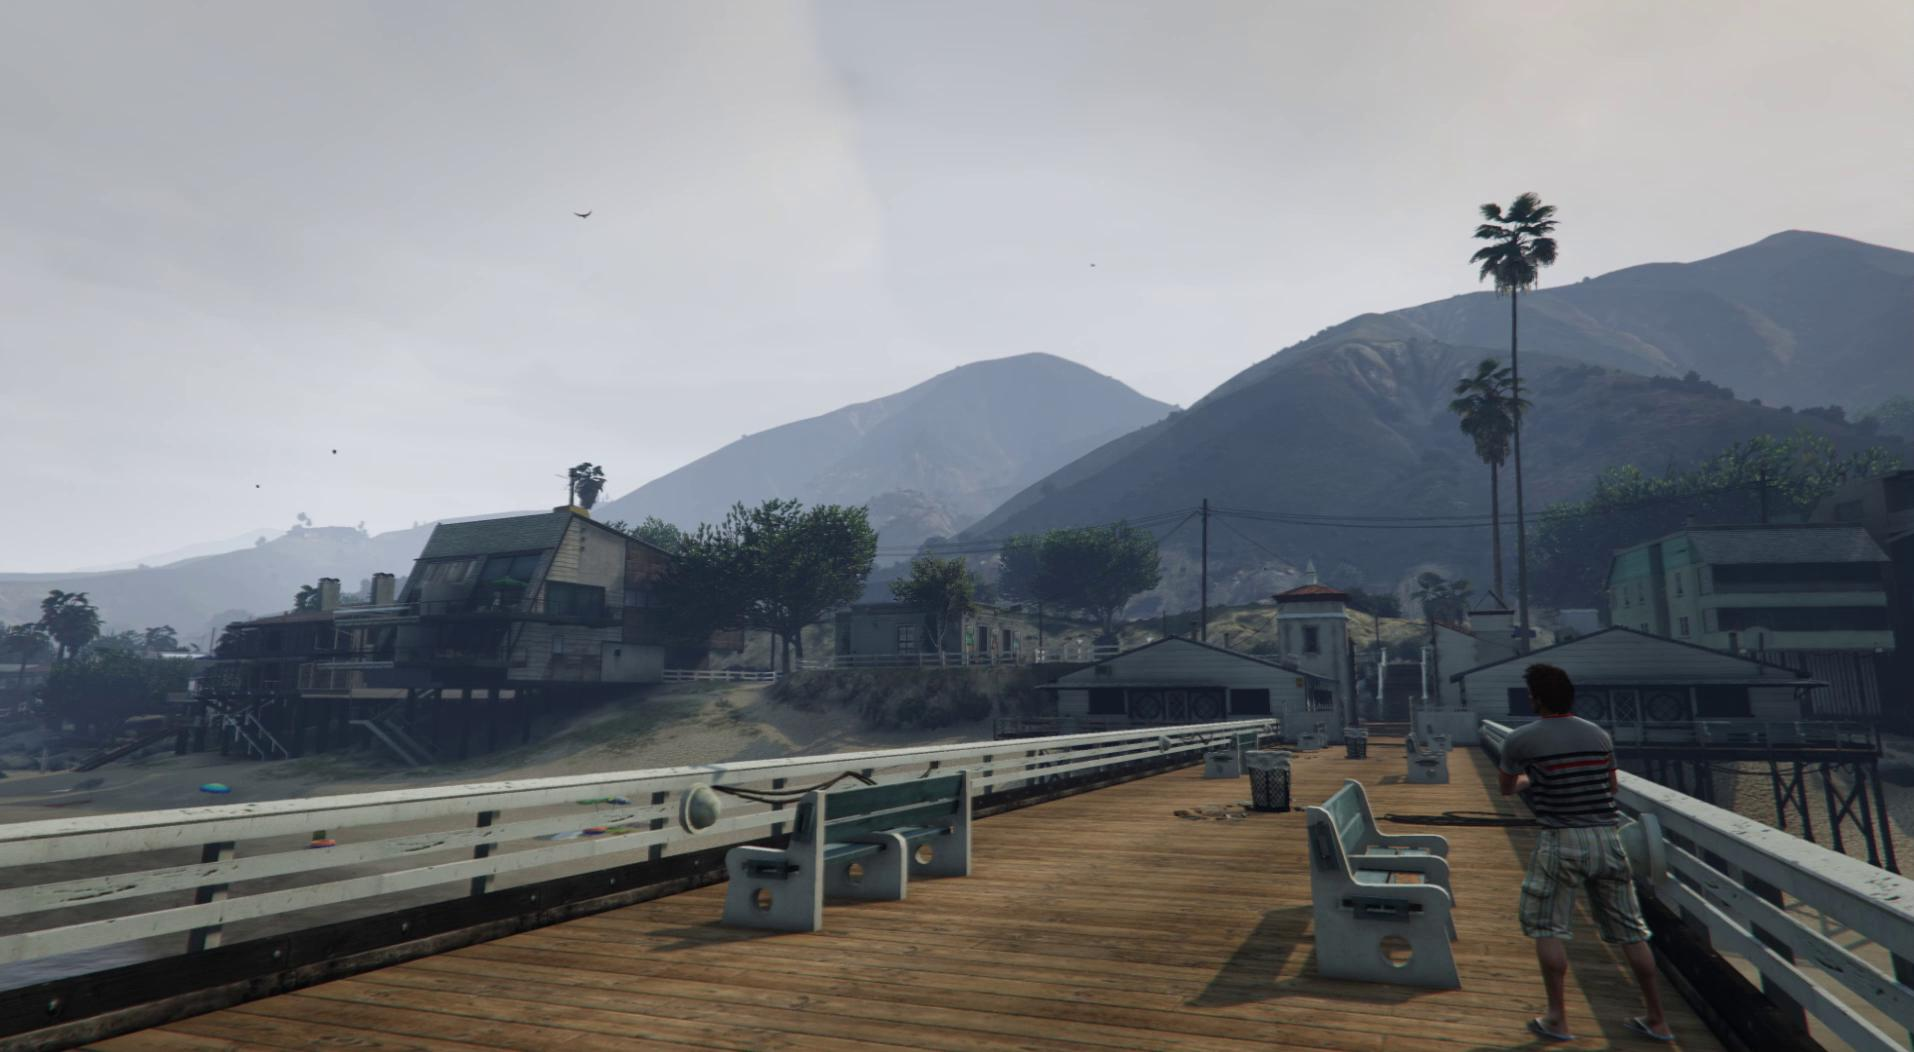
\includegraphics[height=\imheight, width=\imwidth]{Data/GTAV/pier-cloudy}
				\end{subfigure}\hfill%
				\begin{subfigure}[b]{0.33\linewidth}
					\centering
					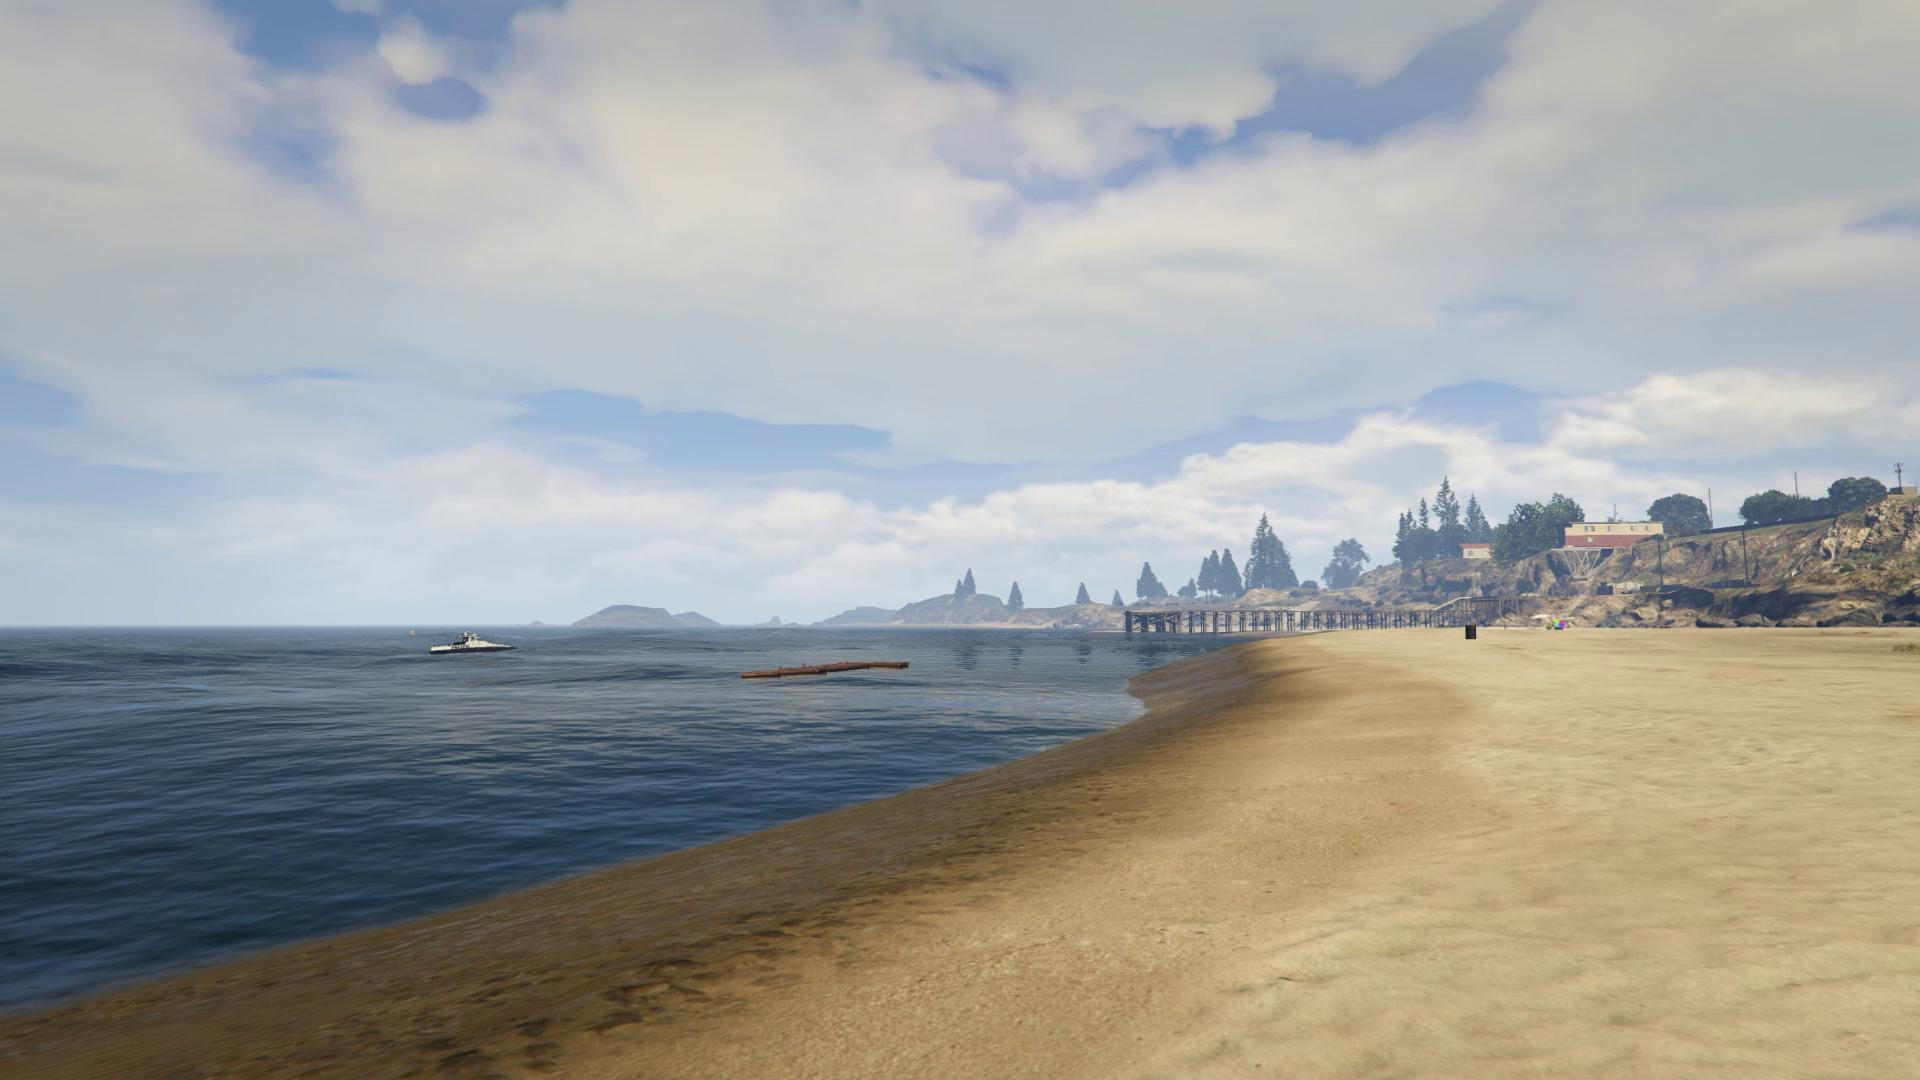
\includegraphics[height=\imheight, width=\imwidth]{Data/GTAV/beach}
				\end{subfigure}\hfill%
				\begin{subfigure}[b]{0.33\linewidth}
					\centering
					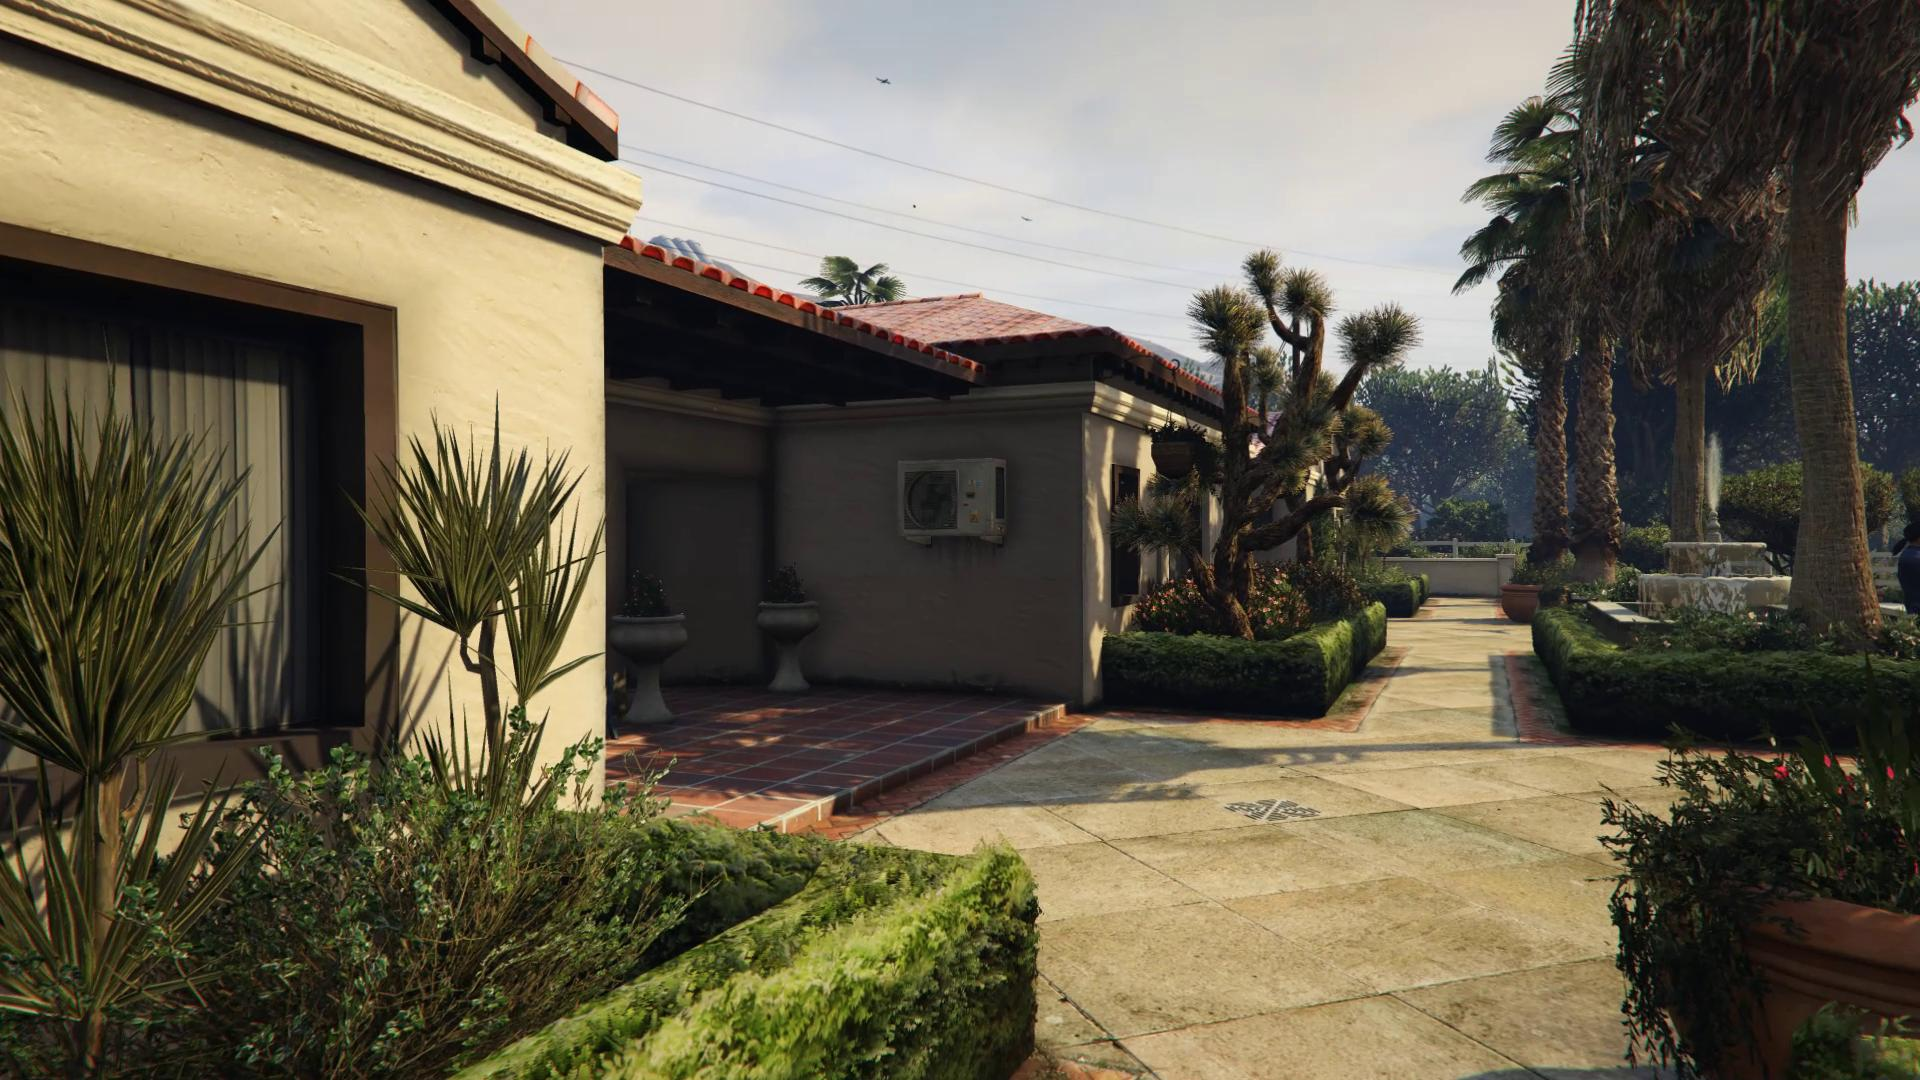
\includegraphics[height=\imheight, width=\imwidth]{Data/GTAV/garden-house}
				\end{subfigure}%
				\\
				\vspace{0.1cm}
				\begin{subfigure}[b]{0.33\linewidth}
					\centering
					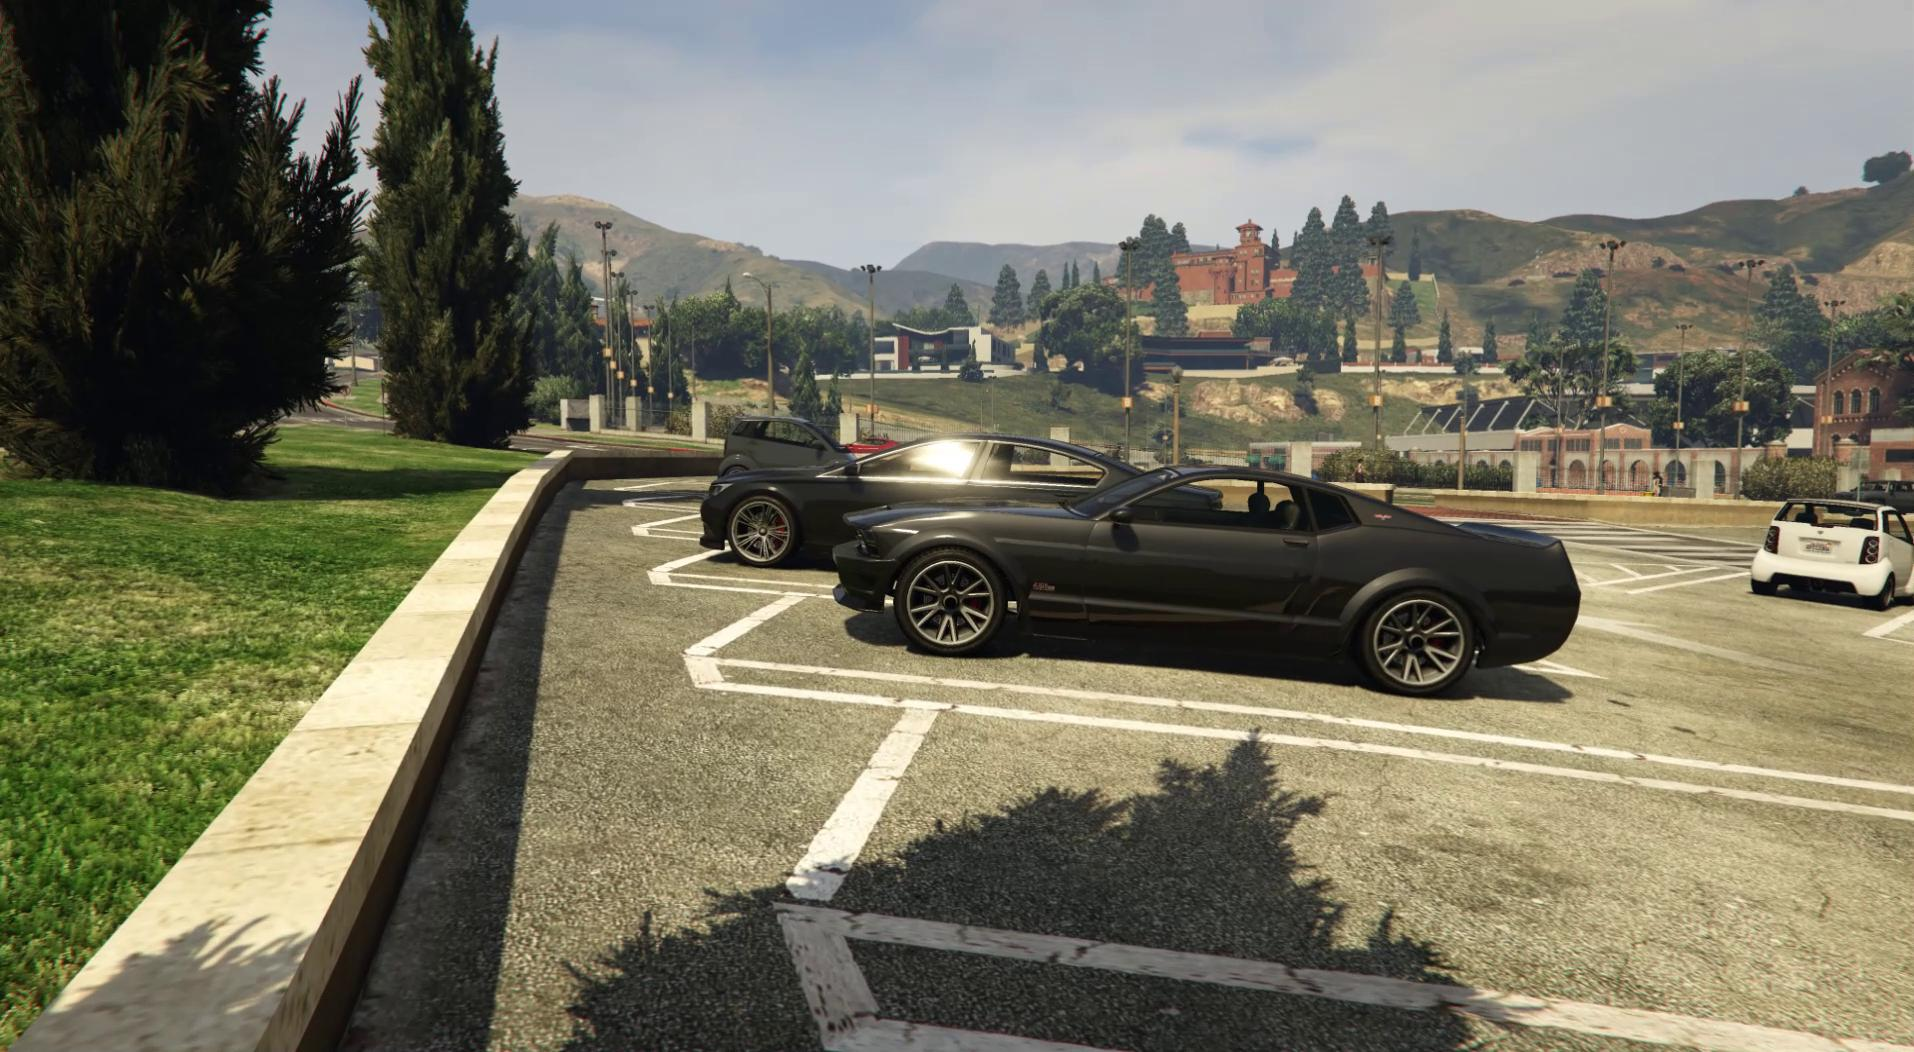
\includegraphics[height=\imheight, width=\imwidth]{Data/GTAV/parked-cars-reflections}
				\end{subfigure}\hfill%
				\begin{subfigure}[b]{0.33\linewidth}
					\centering
					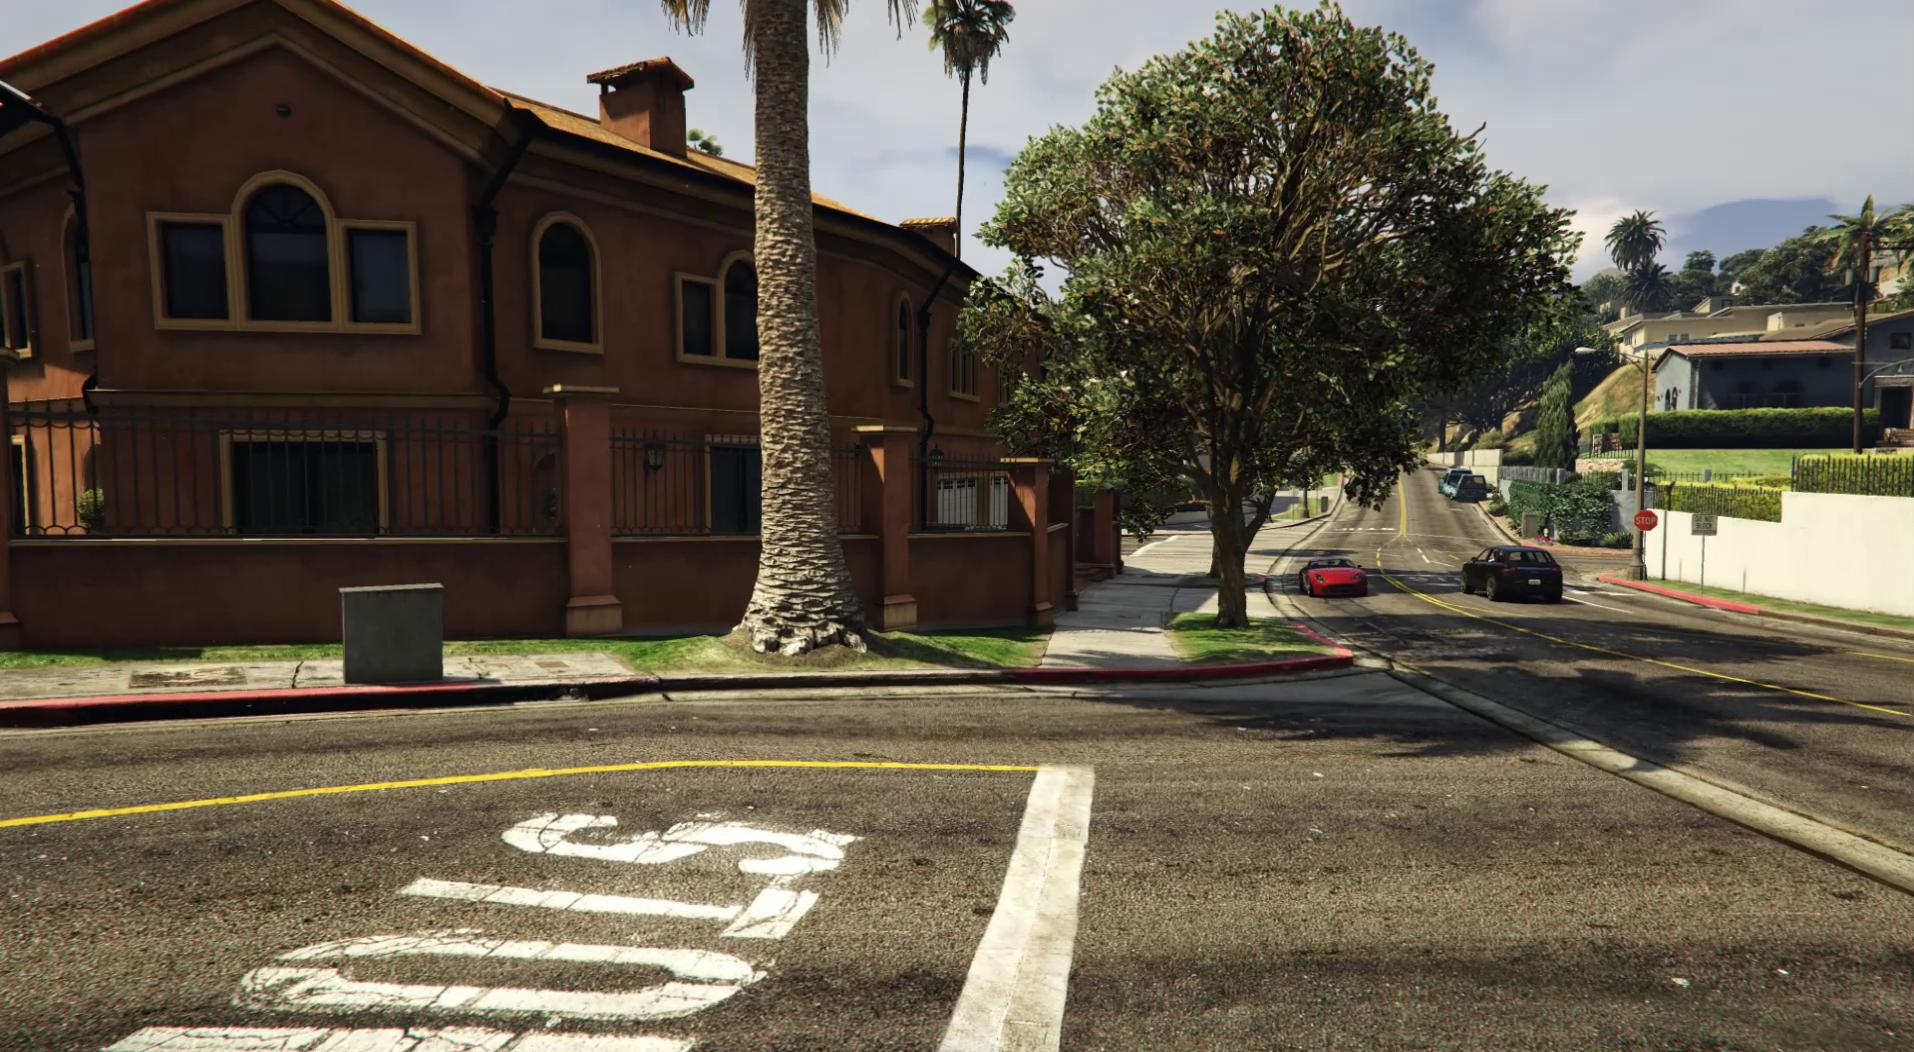
\includegraphics[height=\imheight, width=\imwidth]{Data/GTAV/suburban-sunny-streets}
				\end{subfigure}\hfill%
				\begin{subfigure}[b]{0.33\linewidth}
					\centering
					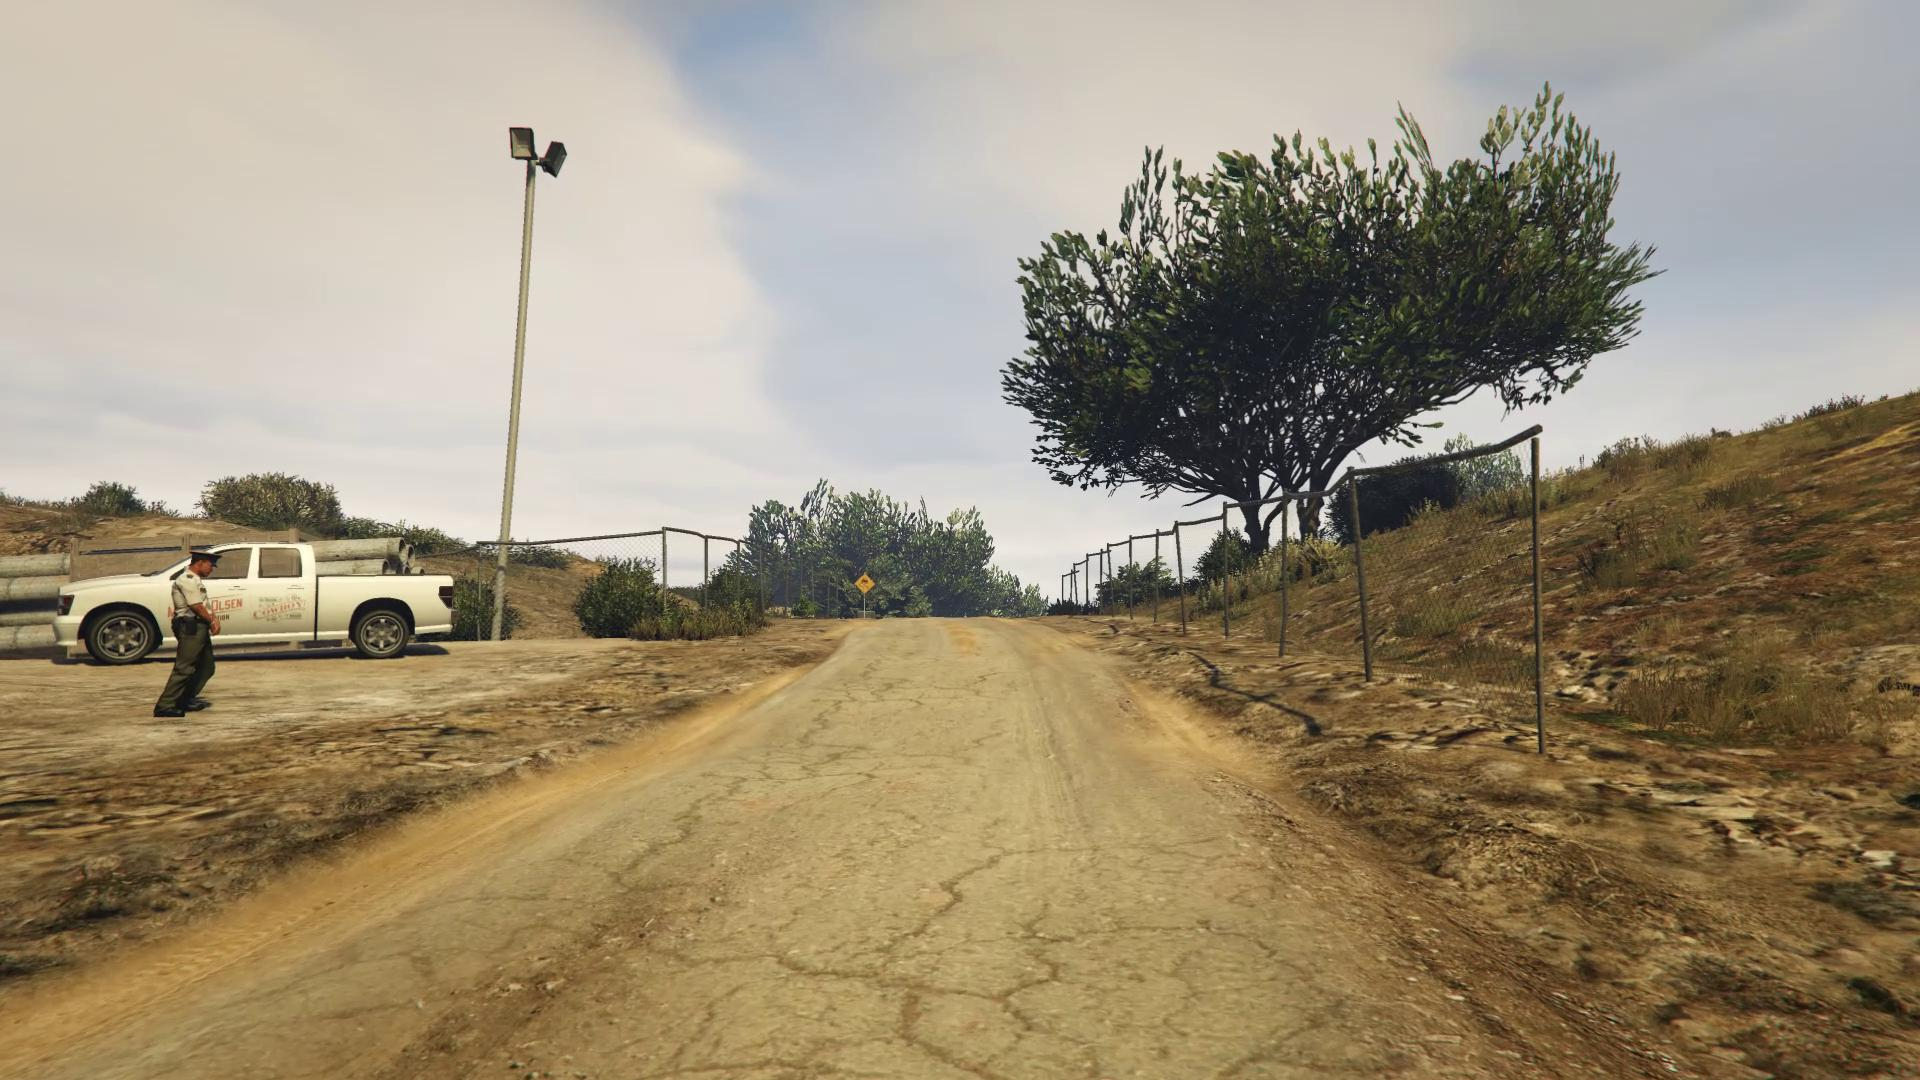
\includegraphics[height=\imheight, width=\imwidth]{Data/GTAV/desert-road}
				\end{subfigure}%
				\vspace{0.1cm}
				\begin{subfigure}[b]{0.33\linewidth}
					\centering
					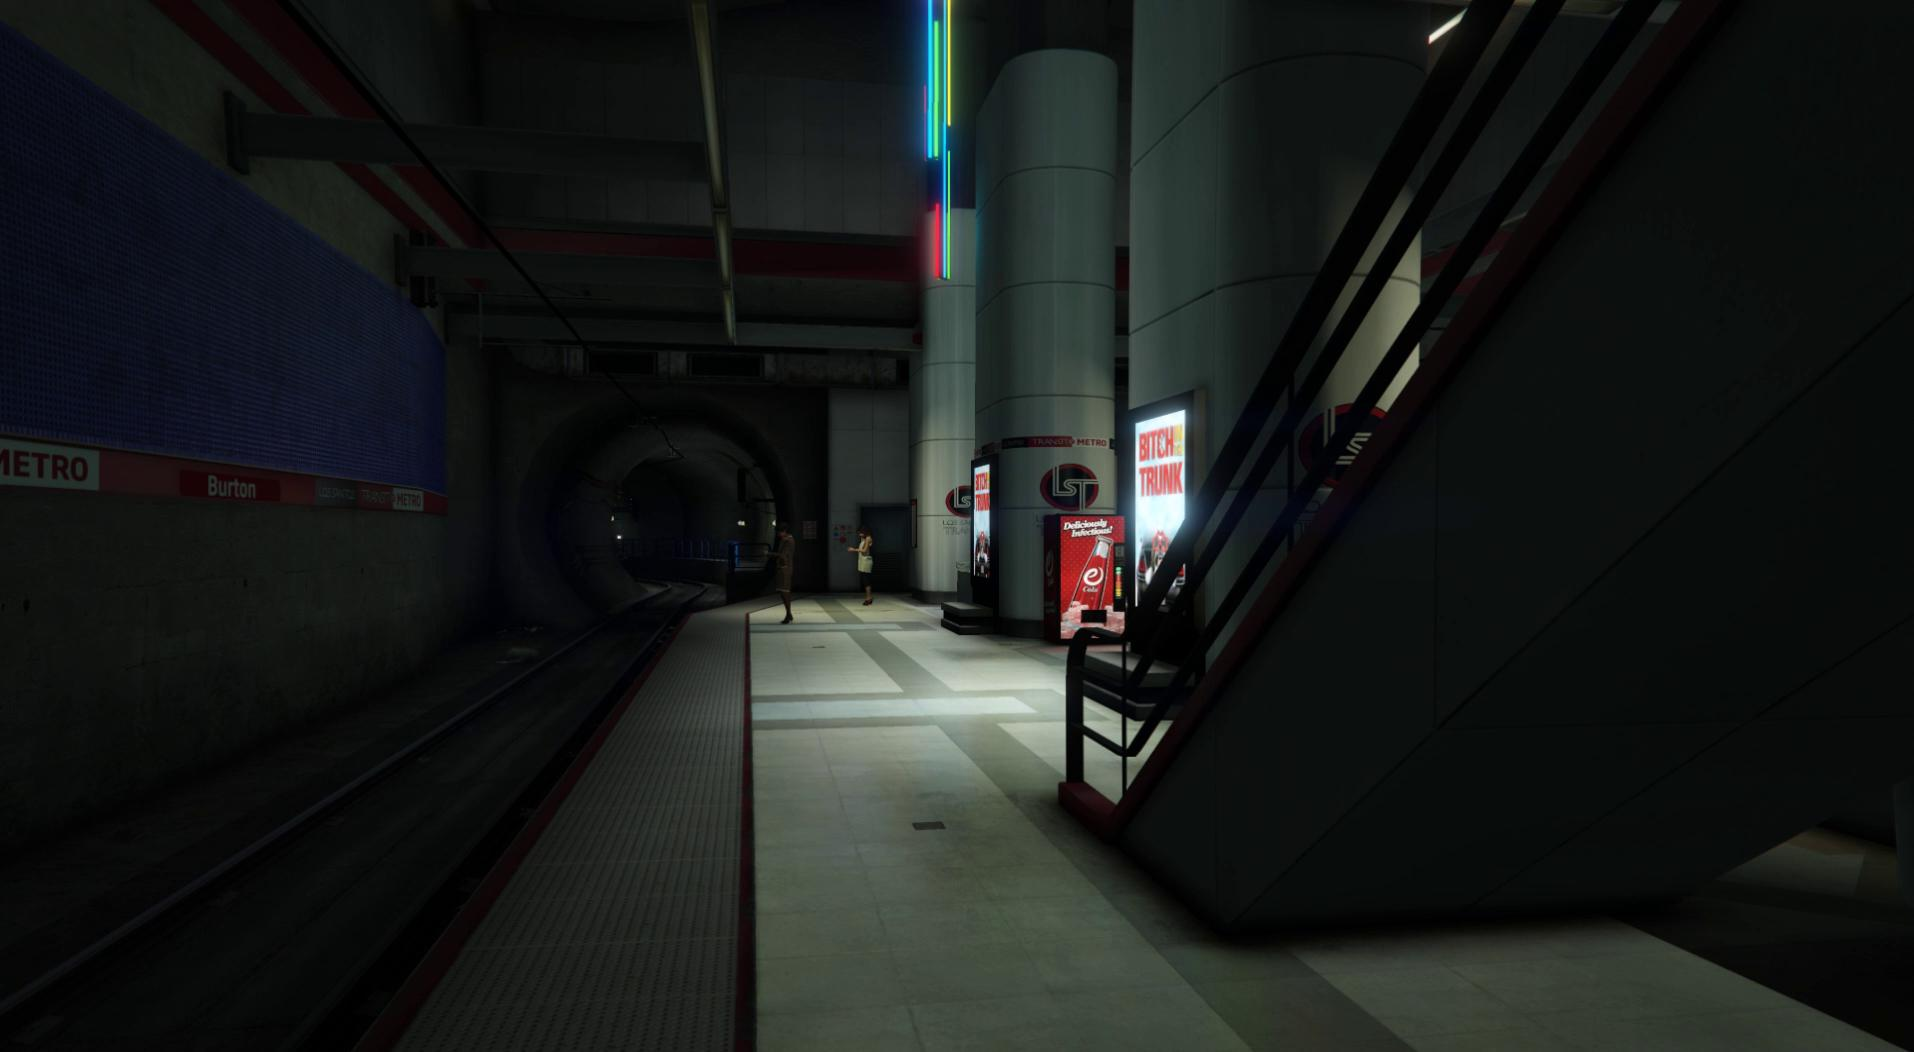
\includegraphics[height=\imheight, width=\imwidth]{Data/GTAV/metro}
				\end{subfigure}\hfill%
				\begin{subfigure}[b]{0.33\linewidth}
					\centering
					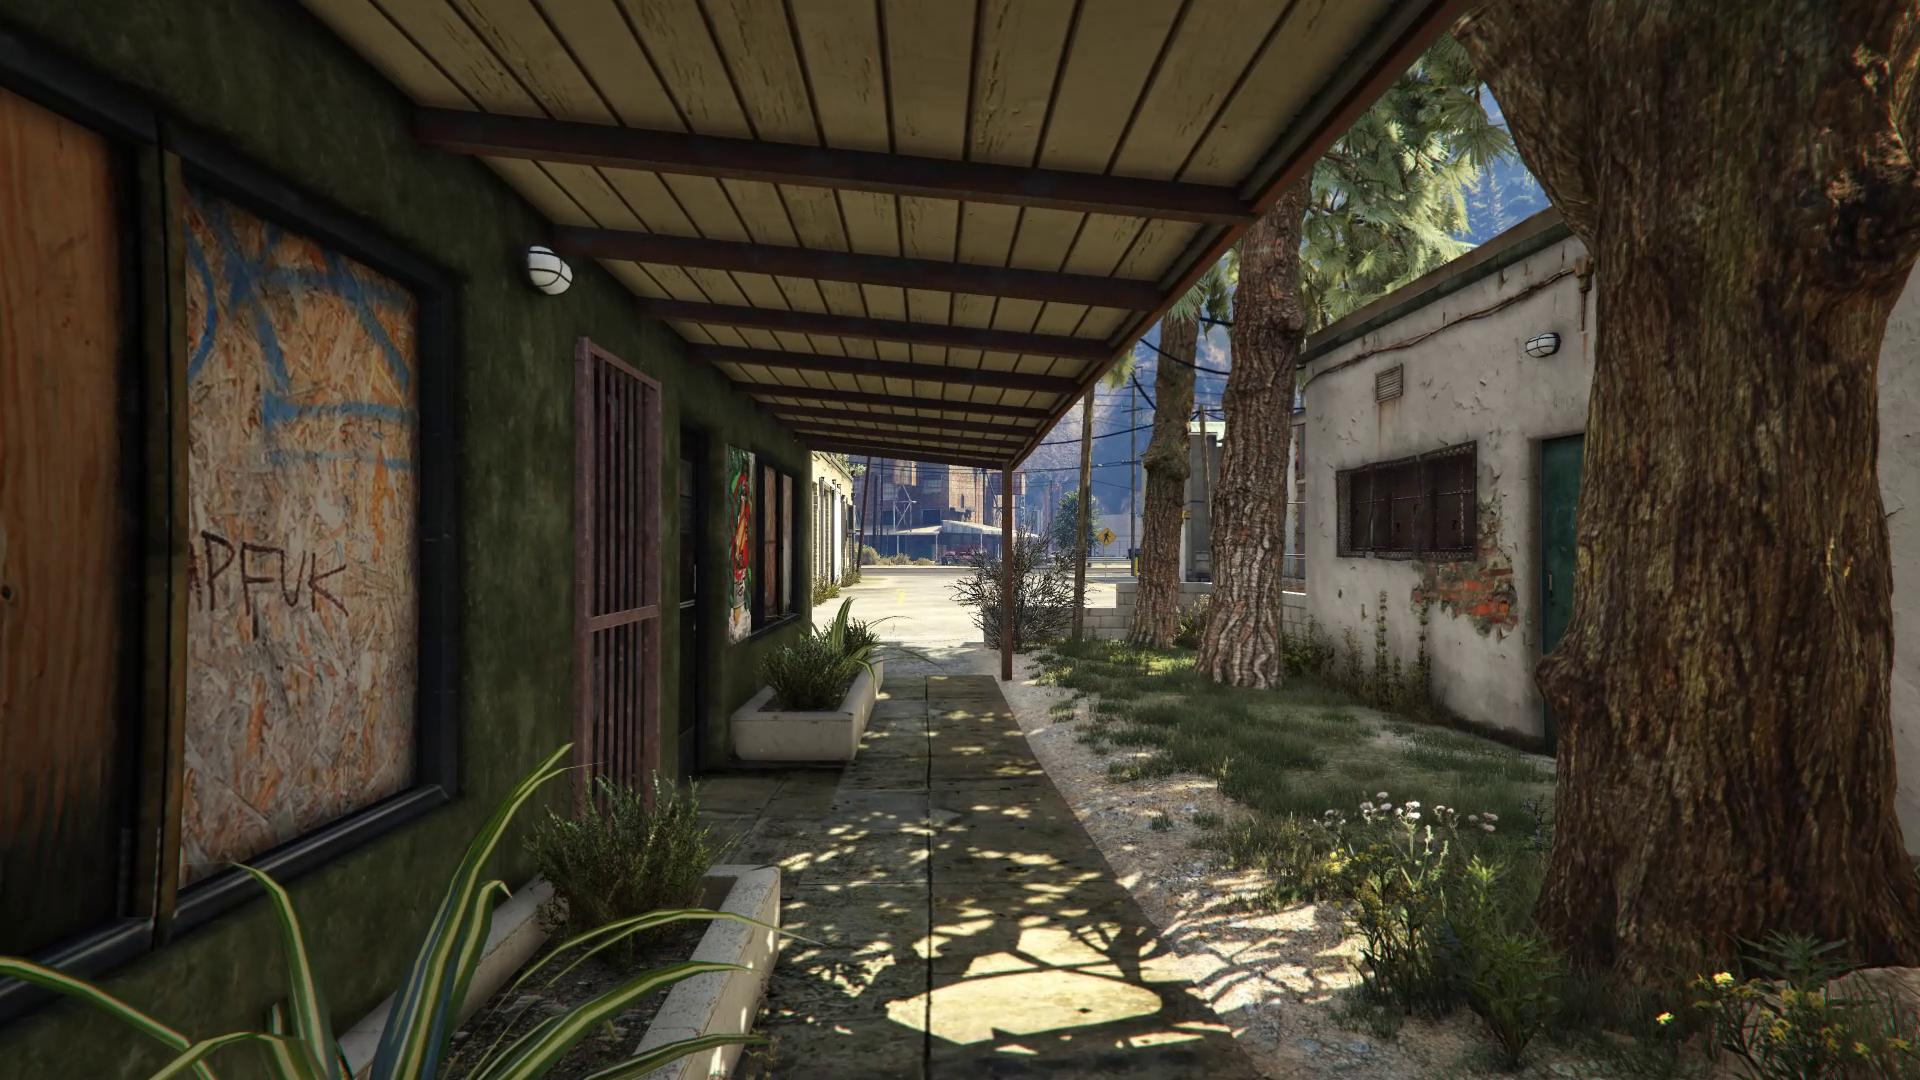
\includegraphics[height=\imheight, width=\imwidth]{Data/GTAV/close-shadows}
				\end{subfigure}\hfill%
				\begin{subfigure}[b]{0.33\linewidth}
					\centering
					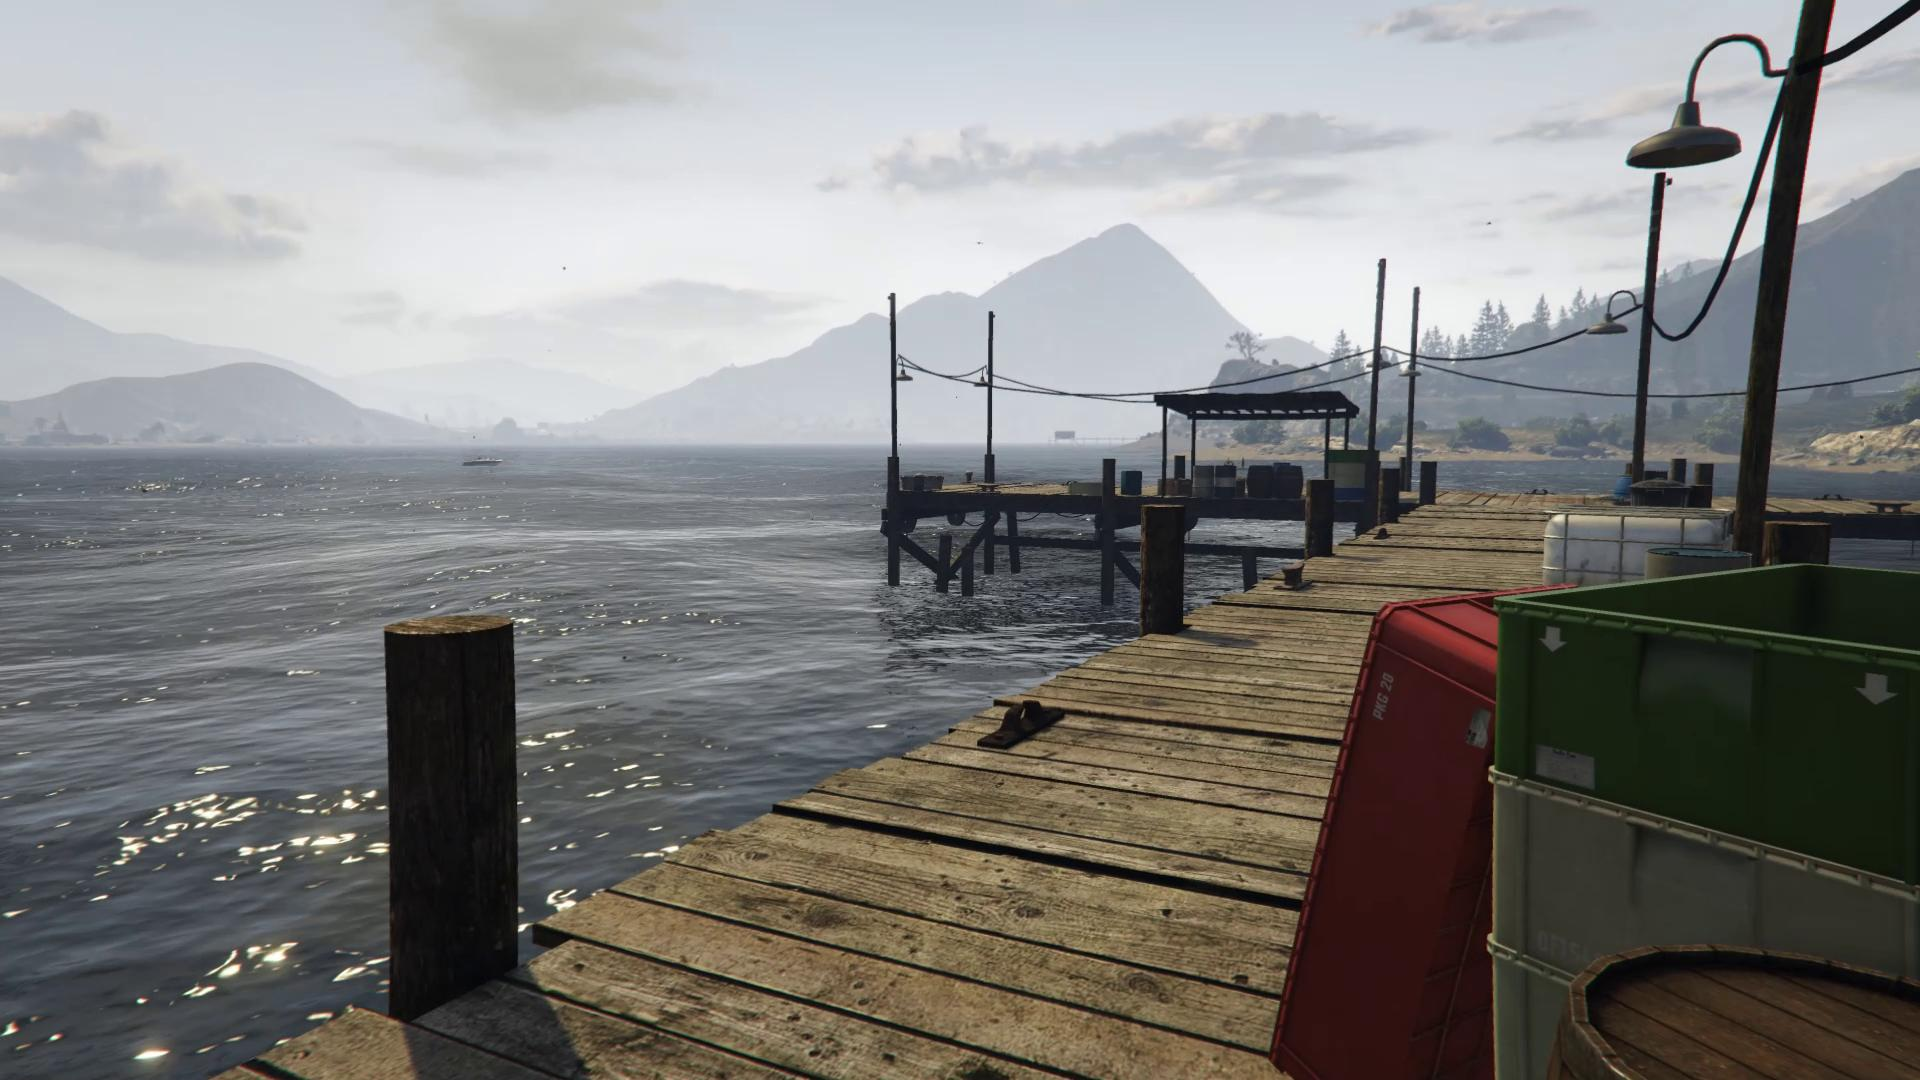
\includegraphics[height=\imheight, width=\imwidth]{Data/GTAV/pier-water-reflections}
				\end{subfigure}%
				\caption[Example images from the GTA V dataset]
						{Example images from different sequences in the GTA V dataset which was recorded for this thesis.
						 The images show wide open- as well as narrow places, reflections on cars and water, complex shadows from foliage and moving objects (people, cars).
						 \label{fig:example-images-GTAV}}
				%city-street-intersecton.jpg  
				%fountain-people.jpg  
				%desert-gas-station.jpg             
				%suburban-intersection.jpg
			\end{figure}
			
			
		\subsection{Preprocessing}\label{sec:preprocessing}
			Each dataset contains long sequences/videos of thousands of frames over several minutes of recording.
			Due to the high memory footprint, it is unfeasible to load a complete sequence and feed it to the network.
			Therefore the sequences are cut into subsequences of smaller sizes. 
			For most experiments here, the sequence size is 100 frames or less.
			Instead of creating a segmentation of the dataset, this method of extracting subsequences also allows to define an overlap between sequences.
			This is especially useful when the dataset is small, such as KITTI.
			
			Since resolution and aspect ratio of the images are different between the datasets, they are first proportionally resized to a height of 320 pixels and then the center region of $448 \times 320$ pixels is extracted.
			Fixing the input size across multiple datasets makes it possible to train the same network architecture for different data and make a more accurate comparison.
			Due to the cropping, the left and right boundaries of the image are removed.
			An alternative is to resize the images directly without regard to the aspect ratio.
			This leads to a loss in horizontal resolution which could impact the networks performance for horizontal motions, e.g., a rotation of the camera around the vertical axis.
			The alternative resizing method was not studied in this thesis, but the impact is expected to be minor.
			
			The ground truth poses also require preprocessing. 
			Each raw sequence has a corresponding text file that contains the $3 \times 4$ pose matrices for every frame.
			These poses are all relative to the coordinate system of the first frame in the sequence.
			In other words, the coordinate system of the first frame is the world coordinate system of all other frames in the sequence.
			Because the raw sequences are divided into subsequences, the ground truth poses need to be converted to poses that are relative to the first frame within each subsequence.
			The formulas in equation~\ref{eq:relative_rotation_conversion_general} from chapter~\ref{chp:foundations} are applied here.
			
			
	\section{Encoding the Pose}
		Each dataset comes with per-frame pose annotations, where each pose is defined by a position and orientation.
		The position always has the same format: It is a vector $\matr{p} \in \R^3$ describing the location of the camera in three-dimensional space.
		As discussed before in chapter~\ref{chp:foundations}, the orientation is a rotation that can be represented in different ways, each having different benefits and use cases.
		Since all representations can be converted between each other, it does not matter in which format the training data is available.
		No matter which representation is chosen, the pose here is always a concatenation of position $\vectr{p}$ and orientation $\vectr{o}$, that is, 
		$\vectr{y} = \left[ \, \vectr{p},  \vectr{o} \, \right]$.
		
		In this work, we investigate two representations for the rotation: Euler angles and unit quaternions.
		In the case of Euler angles, the orientation is defined by the three angles 
		$\vectr{\varphi} = \left[\alpha, \beta, \gamma\right]$, 
		and so the pose is represented as a vector
		$\vectr{y} = \left[ \, \vectr{p},  \vectr{\varphi} \, \right] \in \R^6$ 
		with six degrees of freedom.
		When using unit quaternions, the pose is represented as 
		$\vectr{y} = \left[ \, \vectr{p},  \vectr{q} \, \right] \in \R^7$ 
		where $\vectr{q}$ is a unit-norm quaternion determined by a four-dimensional vector.
		A comparison of how these representations affect the performance is shown in chapter~\ref{chp:experiments-and-results}.
		
	\section{The Model}
	% Figure with the entire pipeline
	% - Figure showing optical flow ??
	% Feature extraction
	%	- Optical flow
	%	- features relevant for motion
	%	- Flow alone is not enough
	% 	- Other high-level representation
	% Pose estimation
	%	- LSTM transforms feature to pose
	%	- Uses history from poses seen before to make current estimate more precise
	%	- 
	% Loss function and optimization
	% mse loss on euler + translation
	% experiments show that euler works best
	% 	
		The model is the key to solving the task.
		By adjusting the weights during the training phase, it learns a high-level representation of relevant information in the input that is needed to produce the desired output.
		In the case of Visual Odometry, we aim to learn a representation for motion.
		Specifically, the network has to be able to distinguish between dynamic motion in the scene and camera motion.
		These and other challenges mentioned in the~\nameref{chp:introduction} chapter are addressed by the two main parts of the model described in the following two sections.
		The architecture of the full model is shown in figure~\ref{fig:main-architecture}.
		\begin{figure}[t]
			\centering
			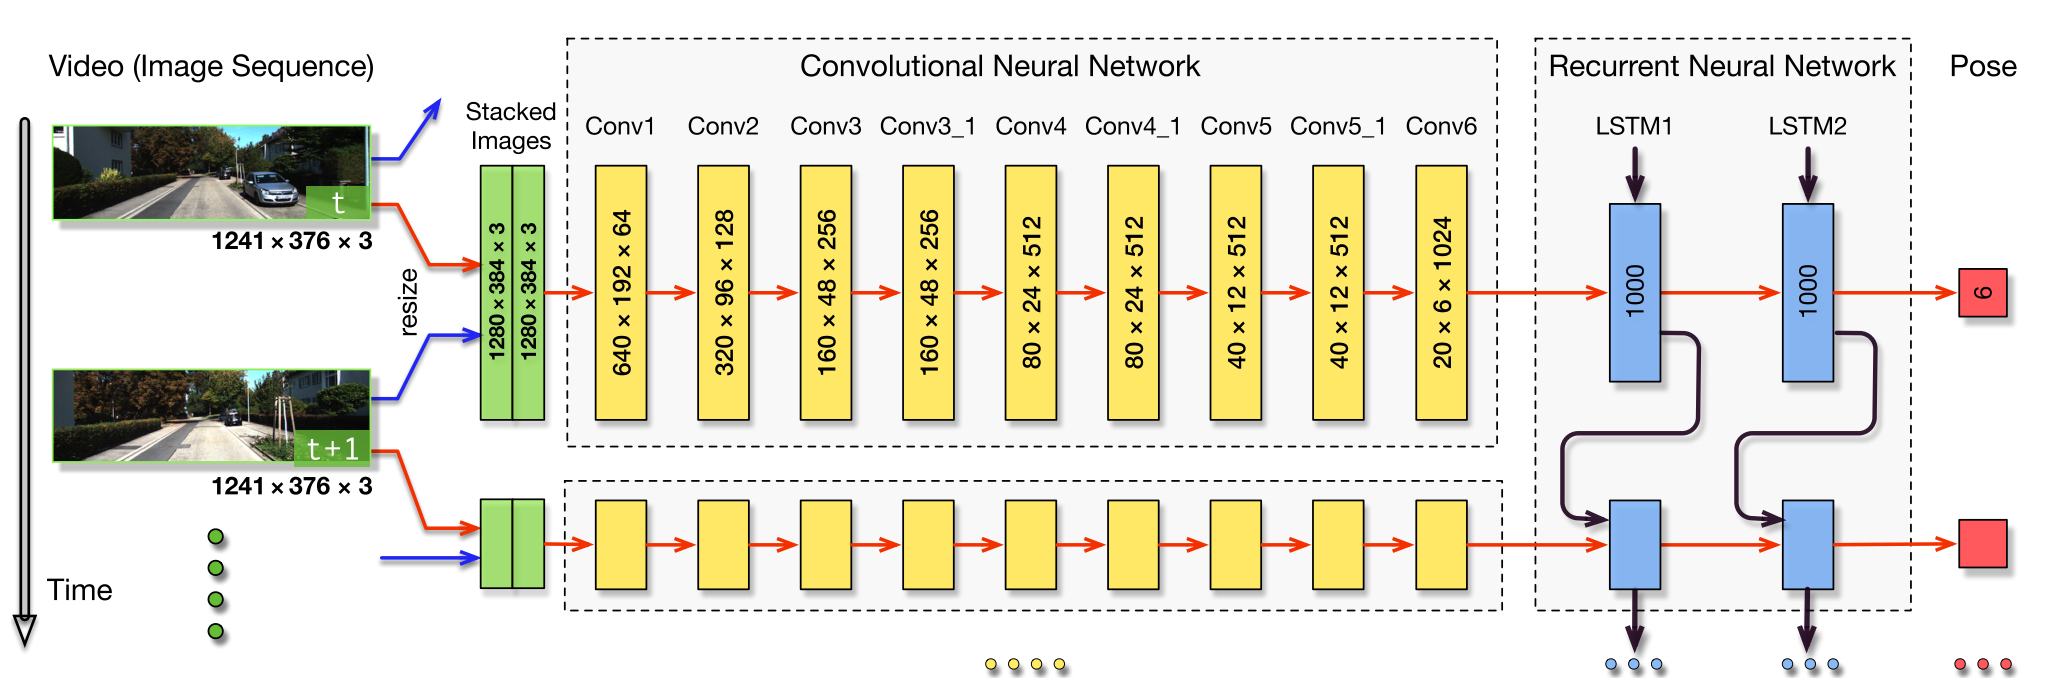
\includegraphics[width=\linewidth]{Model/DeepVO-arch}
			\caption[Main architecture for Visual Odometry]
					{Main architecture for Visual Odometry.
					 Green: Input of consecutive video frames.
					 Yellow: Feature extraction layers.
					 Blue: Pose estimation with recurrent connections.
					 The figure was taken from~\cite{wang2017deepvo}.
					 \label{fig:main-architecture}}
		\end{figure}
		
		\subsection{Part 1: Feature Extraction}
			The purpose of the first part of the network is to extract information about motion from two consecutive frames at time $t$ and $t - 1$.
			One way to describe motion between two images is by \emph{optical flow}.
			It is defined as a vector-valued function $u(\vectr{x}) \in \R^2$ at each point $\vectr{x}$ in the image $I_{t}$ describing the translation of the point in the next frame such that
			\begin{equation}\label{eq:brightness_constancy_constraint}
				I_{t}(\vectr{x}) = I_{t + 1}(\vectr{x} + u(\vectr{x})).
			\end{equation}
			The property in equation~\ref{eq:brightness_constancy_constraint} is called the \emph{brightness constancy constraint}. 
			It means that a particular point can move in the image plane but it does not change its color.
			In general, this constraint does not hold for every point, e.g., because of occlusion introduced by motion.
			
			\cite{dosovitskiy2015flownet} describe a deep-learning approach for estimating optical flow.
			They propose and study two network architectures, \emph{FlowNetS} and \emph{FlowNetC}.
			The later is computing the inner product between patches of two input frames (correlation) followed by multiple layers of convolutions.
			FlowNetS on the other hand is the simple version that does not have the correlation layer. 
			Instead, it is only made of convolution layers and ReLUs.
			The first half of FlowNetS are strided convolutions that gradually increase the number of feature maps. 
			The second half, called refinement, consists of transposed convolution layers that, in reverse, increase the spatial dimension to form the high resolution optical flow maps.
			In addition, both FlowNet versions make use of skip-connections that allow the features from earlier layers to be added as input to layers in the second half by concatenating the tensors along the feature channel dimension. 
			
			In this thesis, the focus is on FlowNetS because it is the only publicly available implementation for PyTorch.%
			\footnote{\citet*{flownetpytorch} has the source code available on GitHub.}
			FlowNetS is also the choice in the work of \citeauthor{wang2017deepvo}, which is the basis of the architecture described here.
			The FlowNetS implementation comes with pre-trained model weights.
			It is trained on a synthetic dataset of moving chairs rendered into images that serve as a static background.
			Although this data does not include camera motion, according to \mbox{\citeauthor{wang2017deepvo}} the model weights serve as a good initialization that leads to faster convergence. 
			
			Estimating camera motion solely based on optical flow is not very robust since scene motion is mixed into the optical flow which can significantly vary in magnitude.
			In order to have a more abstract representation, only the layers in the first half up to ``CONV 6.1'' are used for feature extraction.
			All layers in the second half of FlowNetS are dropped.
			The exact configuration of the remaining layers is shown in table~\ref{tbl:first_part_of_flownets}.
			\begin{table}[tb]
				\small
				\begin{center}
					\begin{tabular}{lcccc}
						\toprule
						Layer 		& Kernel size 		& Stride 		& Padding 		& Channels 		\\
						\midrule
						CONV 1 		& $7 \times 7$		& 2 			& 3 			& 64 			\\
						CONV 2 		& $5 \times 5$		& 2 			& 2 			& 128 			\\
						CONV 3 		& $5 \times 5$		& 2 			& 2 			& 256			\\
						CONV 3.1 	& $3 \times 3$		& 1 			& 1 			& 256 			\\
						CONV 4 		& $3 \times 3$		& 2 			& 1 			& 512 			\\
						CONV 4.1 	& $3 \times 3$		& 1 			& 1 			& 512 			\\
						CONV 5 		& $3 \times 3$		& 2 			& 1 			& 512 			\\
						CONV 5.1 	& $3 \times 3$		& 1 			& 1 			& 512 			\\
						CONV 6 		& $3 \times 3$		& 2 			& 1 			& 1024 			\\
						CONV 6.1 	& $3 \times 3$		& 1 			& 1 			& 1024 			\\
						\bottomrule
					\end{tabular}
				\end{center}
				\caption[Architecture of the feature extraction based on FlownetS]
						{Architecture of the feature extraction based on FlownetS. 
						 Each layer is a convolution followed by a rectified linear unit (ReLU).
						 \label{tbl:first_part_of_flownets}}
			\end{table}
			Note that the convolutions are applied with a stride and therefore the spatial size is reduced from one layer to the next.
			At the same time, the number of feature maps (channels) increases up to 1024 in the last layer.
			Say the input images have a width and height of $448 \times 320$ pixels, for example. 
			Then the output tensor contains 1024 feature maps of size $7 \times 5$.
			These activations are a coarse and abstract description of the motion seen in the input and do not directly imply the per-pixel optical flow.
			To emphasize again, we do not directly make use of optical flow since we are interested in separating camera motion from scene motion.
			This has to be done on a higher level of abstraction.
			The remaining task is now to take these coarse features and map them to the camera pose. 
			
		\subsection{Part 2: Pose Estimation}
		% How does LSTM use flow features 
		% Table with fc layer and dropout
			The key component of the second part is the LSTM that maps the motion features to a hidden state.
			Due to the recurrent connections, the hidden state does not only encode the pose at the current time step, but also a history of poses from previous time steps.
			To be clear, it is not obvious that the LSTM will actually learn a representation for the past and use that information to estimate the pose because nothing is explicitly forcing the network to do so.
			The question whether or not the recurrent connections make a significant contribution will be addressed in chapter~\ref{chp:experiments-and-results}.
			
			As opposed to convolution layers, the LSTM is defined in terms of matrix operations and hence the size of the input to the LSTM is not variable.
			This also implies that there is a limit on the size of the input images.
			As described in section~\ref{sec:preprocessing}, the images are rescaled to $448 \times 320$ pixels, which leads to a tensor of size $1024 \times 7 \times 5$ after feature extraction.
			This tensor is then reshaped to a vector with $1024 \cdot 7 \cdot 5 = 35840$ elements and fed to the LSTM as input.
			Although the LSTM itself applies multiple operations involving input, hidden state and gate outputs, it can be summarized as one single layer.
			Moreover, as shown in figure~\ref{fig:main-architecture} we adopt the architecture of~\citeauthor{wang2017deepvo} and stack two LSTM layers.
			Each of these recurrent layers has an associated hidden state of size $d = 1000$.
			
			The recurrent layers are followed by dropout and a fully connected layer that reduces the output size of the LSTM to a 6D or 7D pose vector depending on the chosen representation.
			Table~\ref{tbl:lstm_and_fc_after_flownet} summarizes the input- and output dimensions of all layers in the second component of the network.
			\begin{table}[tb]
				\small
				\begin{center}
					\begin{tabular}{lcc}
						\toprule
						Layer 		& Input size 					& Output size			\\
						\midrule
						LSTM 1 		& $35840$						& $1000$  				\\
						LSTM 2 		& $1000$						& $1000$ 				\\
						DROP		& $1000$						& $1000$				\\
						FC 			& $1000$						& $6$ or $7$			\\
						\bottomrule
					\end{tabular}
				\end{center}
				\caption[Architecture of the recurrent part of the pose network]
						{Architecture of the recurrent part of the pose network.
						 It consists of a two-layer LSTM with hidden size 1000, a dropout- and fully-connected layer.}
				\label{tbl:lstm_and_fc_after_flownet}
			\end{table}
			The dropout layer is a special layer that randomly overwrites outputs of the previous layer (in this case it is the LSTM) with zeros.
			The fraction of outputs that are kept is controlled by a probability $p \in [0, 1]$, and outputs are ignored with probability $1 - p$.
			By randomly discarding information, the network is forced to learn a redundant representation in order to solve the task.
			In practice, this leads to less overfitting and reduces the test error.
			The effect of dropout for VO is studied in chapter~\ref{chp:experiments-and-results}.
						
	\section{Training}
		Starting from the beginning of a video, the hidden state of the LSTM is initialized with zero.
		Pairs of frames are fed to the CNN that performs the feature extraction as shown in figure~\ref{fig:LSTM-ways-to-use-hidden-state}.
		\begin{figure}[t]
			\centering
			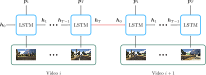
\includegraphics[width=\linewidth]{Foundations/LSTM-hidden-state-loop}
			\caption[Forward operation in time using CNN and RNN]
					{Forward operation in time using the combination of a CNN and RNN. 
					 When using truncated backpropagation, a long video is divided into multiple parts ($i$ and $i + 1$).
					 Between video sequences, one can choose to either transfer the hidden state or reset it.
					 \label{fig:LSTM-ways-to-use-hidden-state}}
		\end{figure}
		At each time step $t$ the LSTM outputs a pose estimate 
		$\vectr{\hat{y}}_t = \left[ \, \vectr{\hat{p}}_t,  \vectr{\hat{\varphi}}_t \right]$ 
		and updates the hidden state $\vectr{h}_t$.
		The quality of the estimated pose is determined by comparison against the ground truth pose 
		$\vectr{y}_t = \left[ \, \vectr{p}_t,  \vectr{\varphi}_t \right]$
		with the loss function
		\begin{equation}\label{eq:euler_pose_loss_function_t}
			\mathcal{L}_t(\vectr{\hat{y}}_t, \vectr{y}_t) = 
			%\sum_{t=1}^{T} 
				\lVert \vectr{\hat{p}}_t - \vectr{p}_t \rVert_2 + 
				\beta \lVert \vectr{\hat{\varphi}}_t - \vectr{\varphi}_t \rVert_2.
		\end{equation}
		As defined in equation~\ref{eq:loss_for_rnn}, the full loss of all estimates in the sequence is the sum of the losses in the sequence, i.e., 
		$\mathcal{L} = \sum_{t = 1}^{T} \mathcal{L}_t$.
		The variable $T$ denotes the number of time steps used for backpropagation.
		Usually, $T$ is fixed before training, and often it is also the length of the input sequences.
		It is still possible to feed videos with length greater than $T$.
		As shown with a red arrow in figure~\ref{fig:LSTM-ways-to-use-hidden-state}, the hidden state can be carried over to the next part of the video instead of resetting it to zero.
		In chapter~\ref{chp:experiments-and-results}, \nameref{chp:experiments-and-results}, we compare the two strategies of how the hidden state is used during training.
		
		
		The loss function in equation~\ref{eq:euler_pose_loss_function_t} balances the squared error of position and Euler angles with a hyperparameter $\beta > 0$.
		The scale of positional change is usually higher than the angular changes for rotation, but in general, the scale depends on the ground truth provided in the dataset, e.g., the unit of measurements used or the speed of the camera motion.
		\cite{kendall2017geometric} find that $\beta$ requires significant tuning to get acceptable results.
		Moreover, as an alternative they propose a loss based on the reprojection error of the 3D points that naturally balances rotation and translation and therefore the need for manual balancing is eliminated.
		However, this thesis does not explore a geometric loss function of this type.
		The balance value in equation~\ref{eq:euler_pose_loss_function_t} is manually chosen and set to $\beta = 10$ by default for training.
		For evaluation on the test set in all experiments that follow, we use $\beta = 1$.
		Furthermore, the two terms 
		$\lVert \vectr{\hat{p}}_t - \vectr{p}_t\rVert_2^2$ and 
		$\lVert \vectr{\hat{\varphi}}_t - \vectr{\varphi}_t \rVert_2^2$
		in equation~\ref{eq:euler_pose_loss_function_t} are referred to as the translation- and rotation errors respectively.
		
		Alternatively, for experiments where the rotations are represented by quaternions, the loss is defined as
		\begin{equation}\label{eq:quaternion_pose_loss_function_t}
			\mathcal{L}_t(\vectr{\hat{y}}_t, \vectr{y}_t) = 
			%\sum_{t=1}^{T} 
			\lVert \vectr{\hat{p}}_t - \vectr{p}_t \rVert_2 + 
			\beta (1 - (\vectr{\hat{q}}_t \cdot \vectr{q}_t)^2)
		\end{equation}
		where $\cdot$ is the inner product of the two unit quaternions.
		The output quaternion of the network is not constraint to have unit-norm and thus, the output needs to be normalized in an additional step before applying the loss function.
		The inner product between the two unit quaternions is equal to the cosine of the angle between the two vectors representing the quaternions on the 4D unit sphere.
		The square in equation~\ref{eq:quaternion_pose_loss_function_t} is necessary to eliminate the sign, because the two quaternions $\vectr{q}$ and $-\vectr{q}$ represent the same rotation.
		Alternatively, the absolute value $\lvert \vectr{\hat{q}}_t \cdot \vectr{q}_t \rvert$ could also be used for this purpose.
		
		The optimizer used to train the model is Adam (\cite{kingma2014adam}).
		Adam (Adaptive Moment Estimation) is an extension of the gradient descent method described in chapter~\ref{chp:foundations}.
		It uses adaptive learning rates for each individual parameter in the network.
		The learning rates are updated based on an exponentially decaying average of past gradients and squared gradients.
		
		The Adam optimizer is applied independently to each part of the network with different initial learning rates
		$\lambda_1 = 10^{-4}$ and $\lambda_2 = 10^{-3}$.
		$\lambda_1$ is the learning rate for the part that is initialized with weights from the pre-trained FlowNetS.
		It is chosen to be smaller than $\lambda_2$ because the transferred weights are expected to be already close to optimal values and can be fine-tuned with a smaller learning rate.
		
		The choice of Adam over other optimizers that use adaptive learning rates (e.g.\@ Adagrad, RMSProp, etc.) is rather arbitrary.
		The main reason why it was chosen in this thesis is to eliminate the need for manual scheduling of learning rate decay over time.
		Without reducing the learning rate, there is a high risk of an oscillation as the parameters approach a local minimum, and this would lead to a slower convergence.

	\section{Implementation}
		The model and training procedure described above is implemented in Python using the deep learning framework PyTorch\footnote{\url{http://pytorch.org}}.
		This framework comes with a rich tensor library with GPU support for all tensor operations. 
		PyTorch differs from other frameworks like TensorFlow, Caffe, or Theano in the sense that it builds the computational graph dynamically at runtime.
		This flexibility allows for dynamic control of computational flow while training or testing the network.
		
		Figure~\ref{fig:code-structure} shows the structure of the code developed for this thesis.
		\begin{figure}[t]
			\centering
			\includegraphics[width=0.9\linewidth]{Implementation/code-structure}
			\caption[Structure of the implemented software]
					{Structure of the implemented software.
					 The main program is broken down into training and testing.
					 Separate data loading classes for each dataset take care of converting the data into the desired format.}
			\label{fig:code-structure}
		\end{figure}
		The main program is split into training and testing.
		It has the responsibility to parse and initialize parameters provided by the user, load and save checkpoints, and create a folder structure for output files like plots and log-files.
		The training and testing code accesses data loading classes and model classes depending on which experiment is conducted.
		Adding a new dataset only requires the implementation of a class for loading and converting the data to the desired format.